\section{\datanamen: Scaling Tool-Agentic Data with Real World MCPs}
\label{sec:toucan-overview}

\begin{wrapfigure}{r}{0.37\textwidth}
  \vspace{-4.5em}
  \centering
  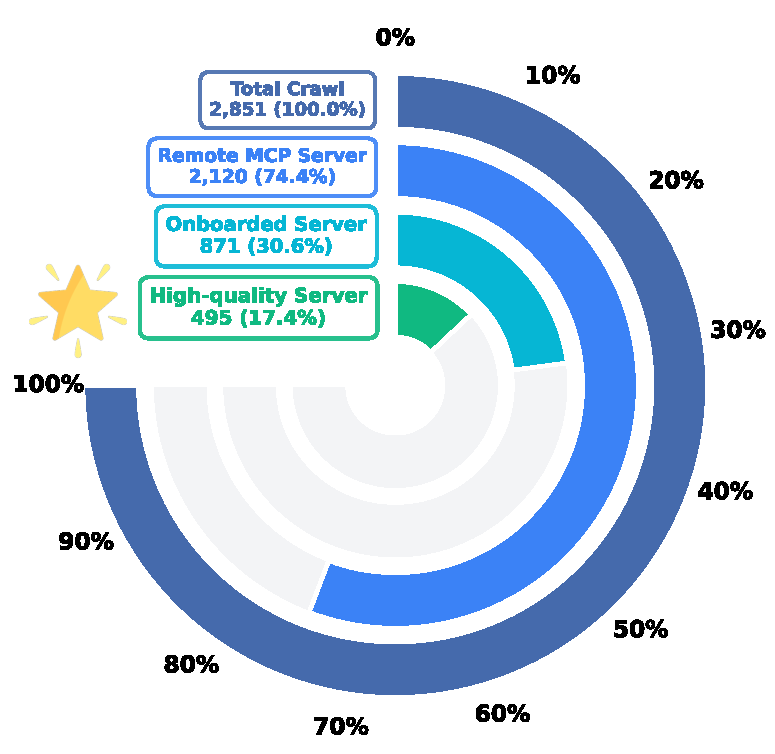
\includegraphics[width=\linewidth]{images/server_num.pdf}
        \caption{MCP servers filtering process}
        \label{fig:server-num}
  \vspace{-2.5em}
\end{wrapfigure}

\subsection{\dataname Generation Pipeline}
\dataname is a comprehensive dataset comprising over 1.5 million tool-agent trajectories constructed using real-world tools from MCP servers. Each instance in our dataset contains a task description, a complete agent trajectory with its associated tools, quality and classification annotations, as well as comprehensive metadata. Appendix~\ref{app:dataset-schema} provides a detailed schema description and demonstration samples.
The construction of \dataname follows a systematic five-stage pipeline: MCP server onboarding, task synthesis, task filtering, trajectory generation, and trajectory filtering. Additionally, we implement three extension mechanisms to further enhance data diversity and realism. Figure~\ref{fig:toucan-mcp-pipeline} illustrates the complete construction pipeline. We detail each stage below.

% Our pipeline first produces a broad spectrum of tool-use tasks using five distinct models, applies model-based quality filtering, then generates agentic trajectories with three teacher models. Rigorous rule and model-based checks ensure high-quality outputs.

\begin{figure}[t!]
    \centering
    % \vspace{-1em}
    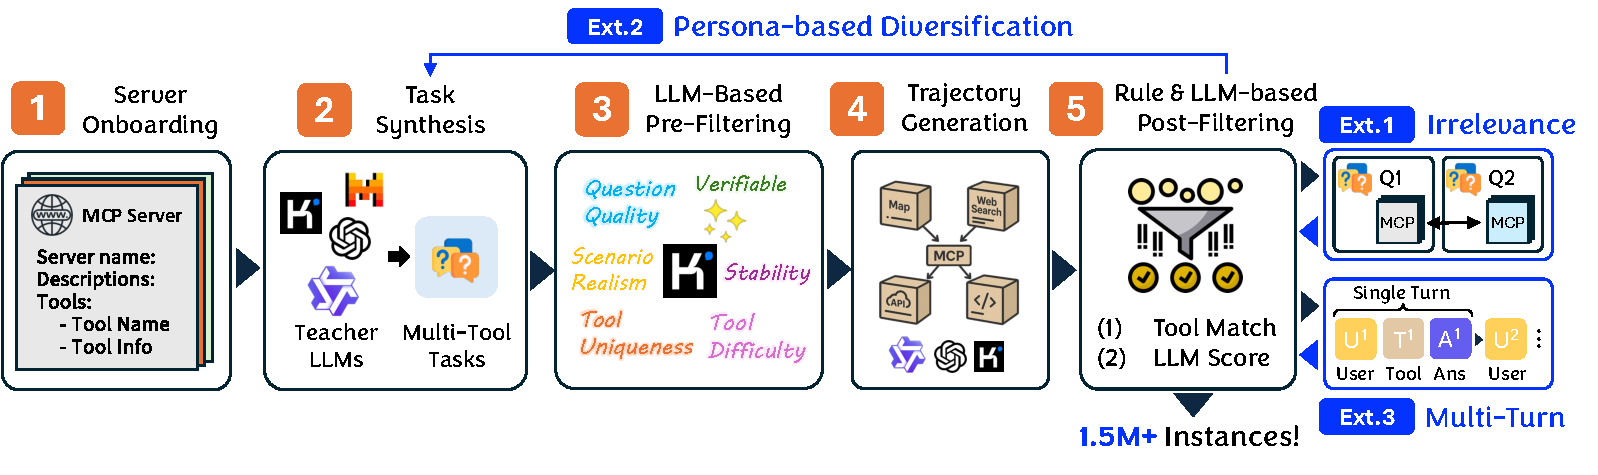
\includegraphics[width=1.0\linewidth]{images/toucan_pipeline_0924.pdf}
    \vspace{-1em}
    \caption{The \dataname construction pipeline: A systematic five-stage process from MCP server onboarding through trajectory filtering, with three extensions for enhancing data diversity and realism.}
    \label{fig:toucan-mcp-pipeline}
    \vspace{-1em}
\end{figure}

\textbf{\textcolor{orange!90!black}{Stage 1: MCP Server Onboarding.}}
%  \begin{itemize}
%     \item Crawling
%     \item Filtering: rule-based (connectivity and stability check, onboarding without special configurations)
%     \item MCP Server category annotation
% \end{itemize}
To generate questions from diverse environments, the initial step involves onboarding as many high-quality MCP servers as possible. We sourced MCP server specification files from GitHub and Smithery \footnote{https://smithery.ai/}, a platform and registry for MCP servers that encapsulate modular execution environments. Each MCP server is accompanied by a structured JSON document detailing metadata about the server with a machine-readable definition of the tools it provides. From an initial crawl yielding approximately 2,800 MCP servers, we applied two key filtering criteria: (1) retaining only remote MCP servers accessible via streamable HTTP to ensure compatibility with trajectory generation, and (2) excluding servers requiring third-party credentials (e.g., API keys) for tool invocation to maintain accessibility and reproducibility. This process reduced the dataset to 30.6\% (871 servers). As a final step, we generated a small subset of test questions to evaluate each tool within the MCP servers, subsequently filtering out servers with problematic tools that returned error messages or failed to function correctly. This rigorous curation process resulted in a refined set of 495 high-quality MCP servers spanning diverse domains and functionalities.
Figure~\ref{fig:server-num} depicts the number of MCP servers retained at each filtering stage. Figure \ref{fig:mcp-servers-category} demonstrates the domain distribution of the final server collection across diverse categories. The domain distribution is annotated by LLMs, where prompts can be found in Appendix \ref{app:server-category-annotation-prompt}.

% \begin{figure}[t!]
% \vspace{-2em}
%     \centering
%     \begin{subfigure}[t]{0.34\textwidth}
%         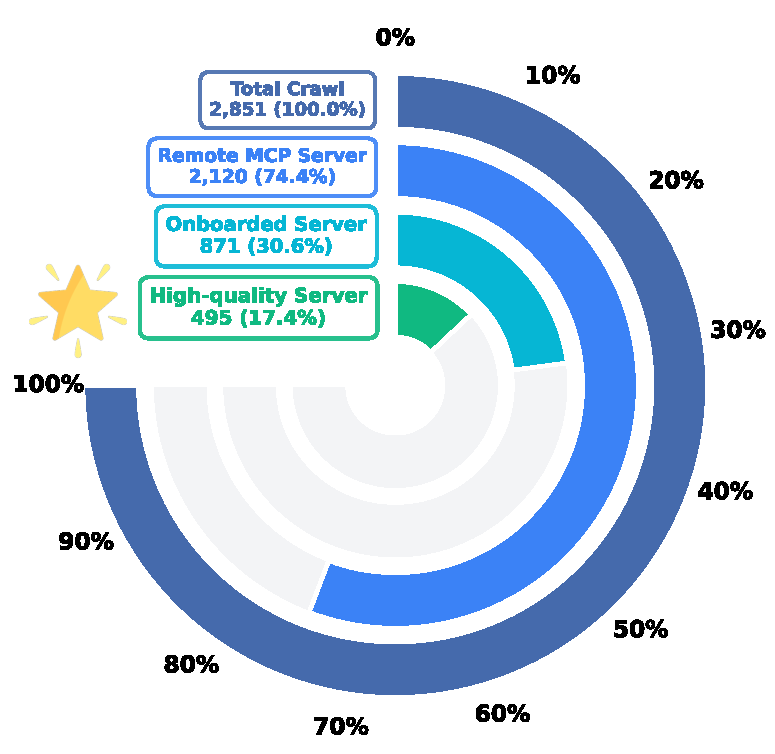
\includegraphics[width=\linewidth]{images/server_num.pdf}
%         \caption{MCP servers filtering process}
%         \label{fig:server-num}
%     \end{subfigure}
%     \hfill
%     \begin{subfigure}[t]{0.33\textwidth}
%         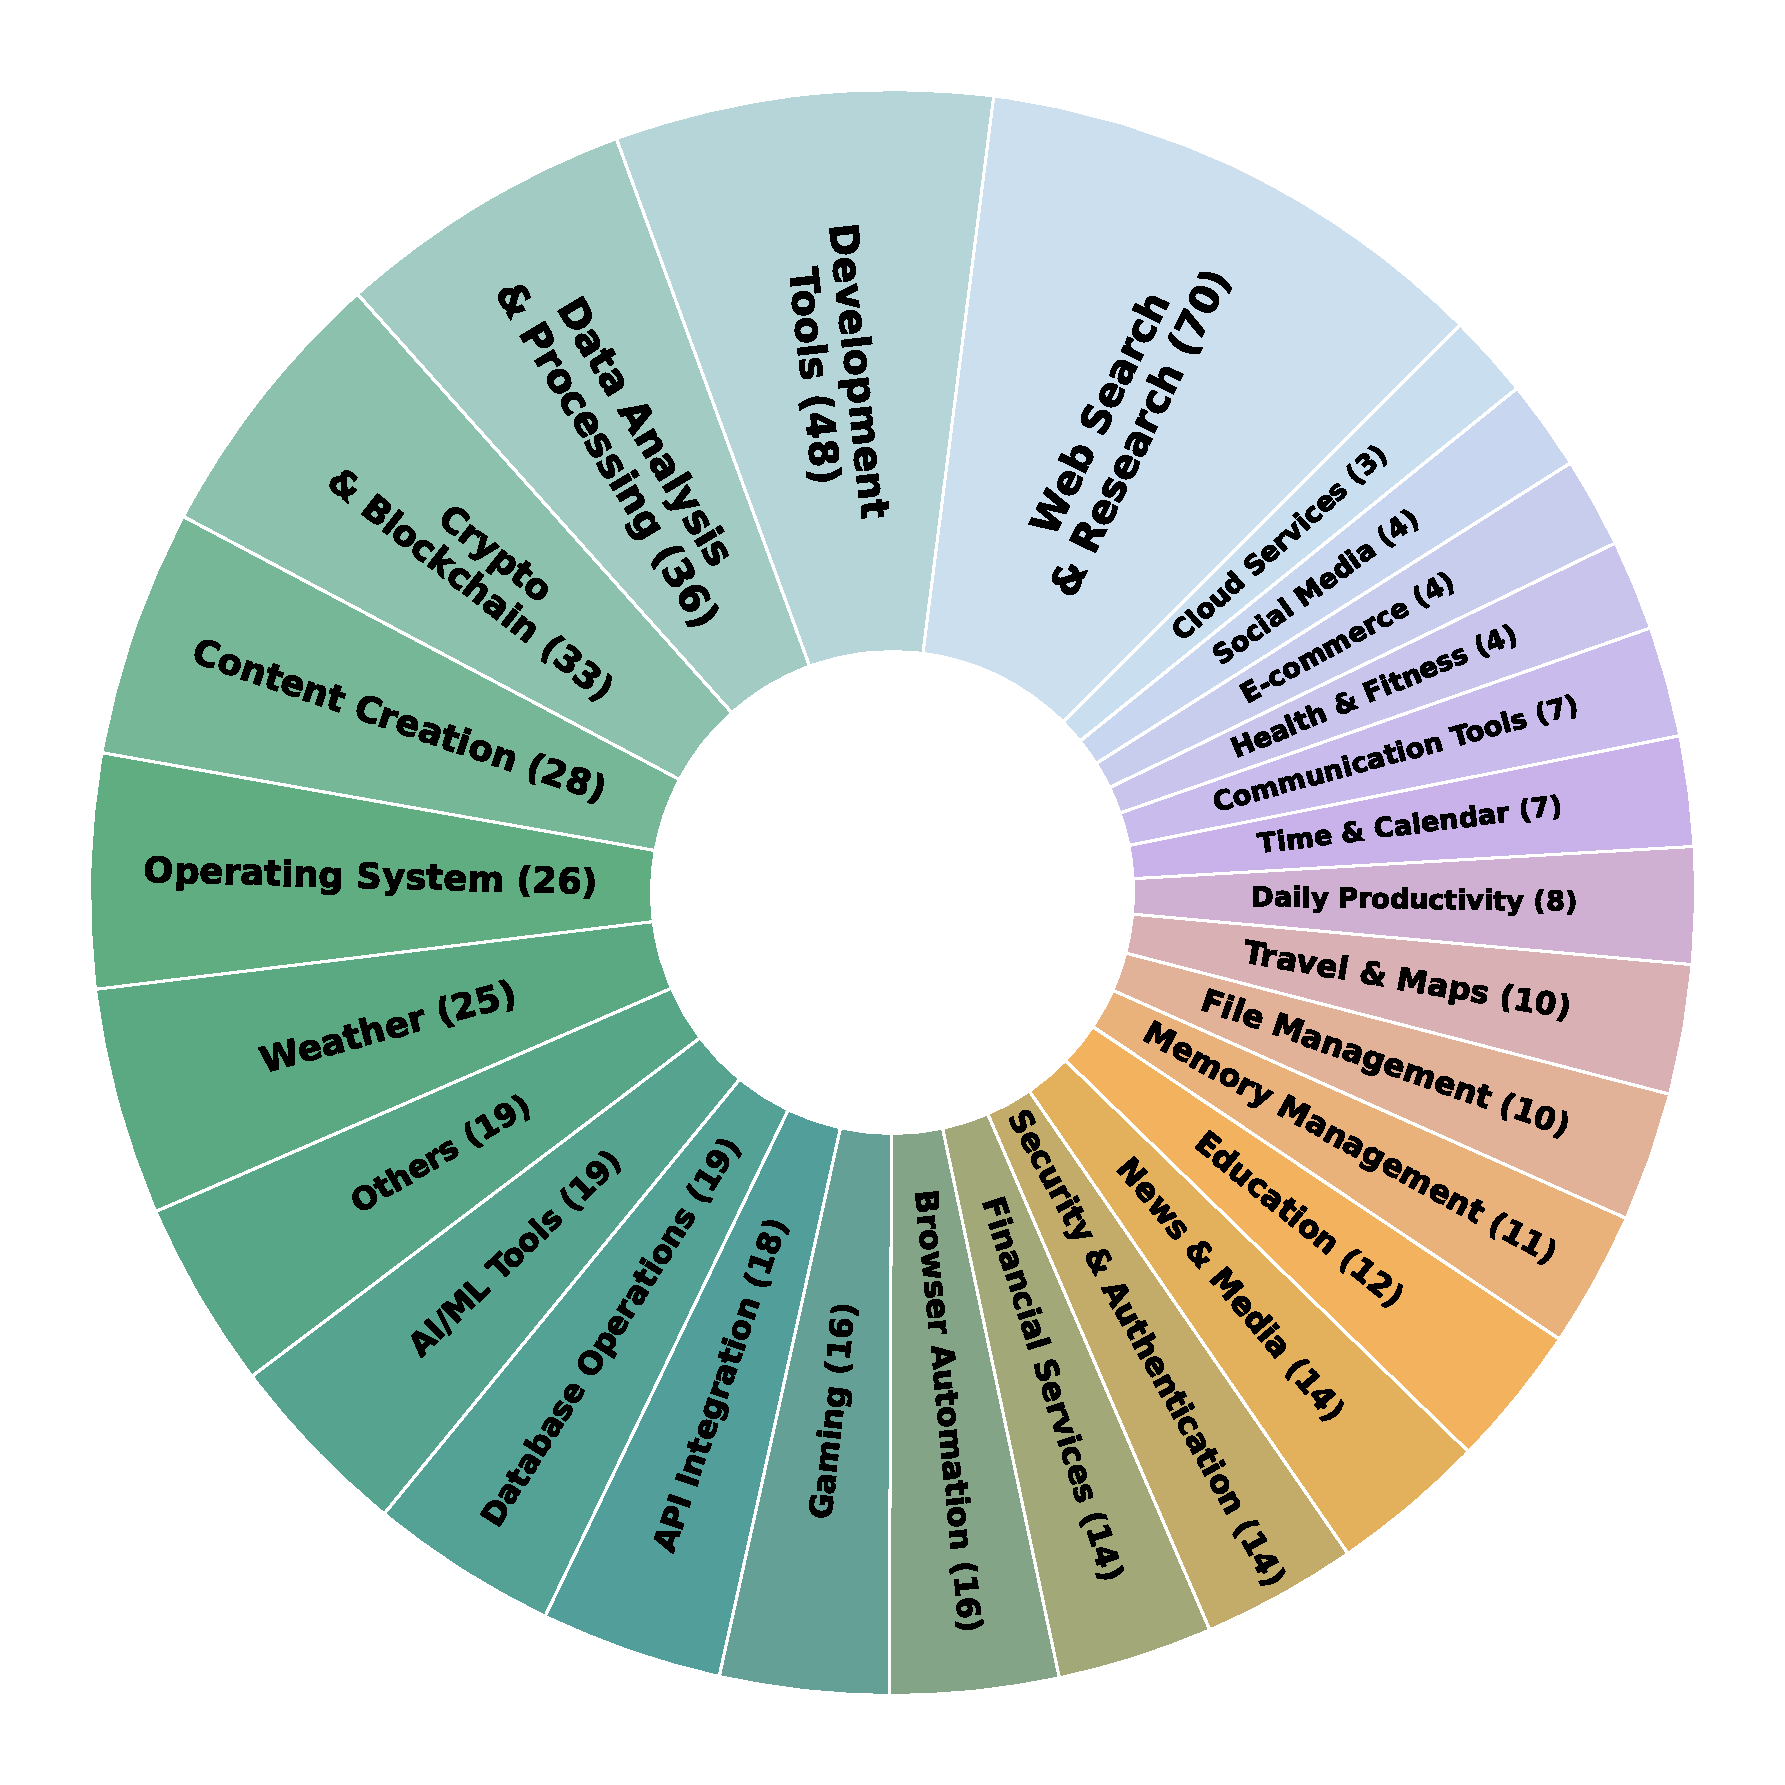
\includegraphics[width=1.0\linewidth]{images/mcp_primary_labels_ring_internal.pdf}
%         \caption{MCP servers distribution by domain}
%         \label{fig:mcp-servers-category}
%     \end{subfigure}
%     % \caption{MCP servers analysis: (a) summarizes MCP servers filtering process, (b) MCP servers distribution by domain, (c) tools number distribution per MCP server.}
%     \caption{Overall statistics of \dataname dataset.}
%     \vspace{-2em}
%     \label{fig:mcp-servers-analysis}
% \end{figure}

\begin{wrapfigure}{r}{0.43\textwidth}
  \vspace{-1.8em}
  \centering
  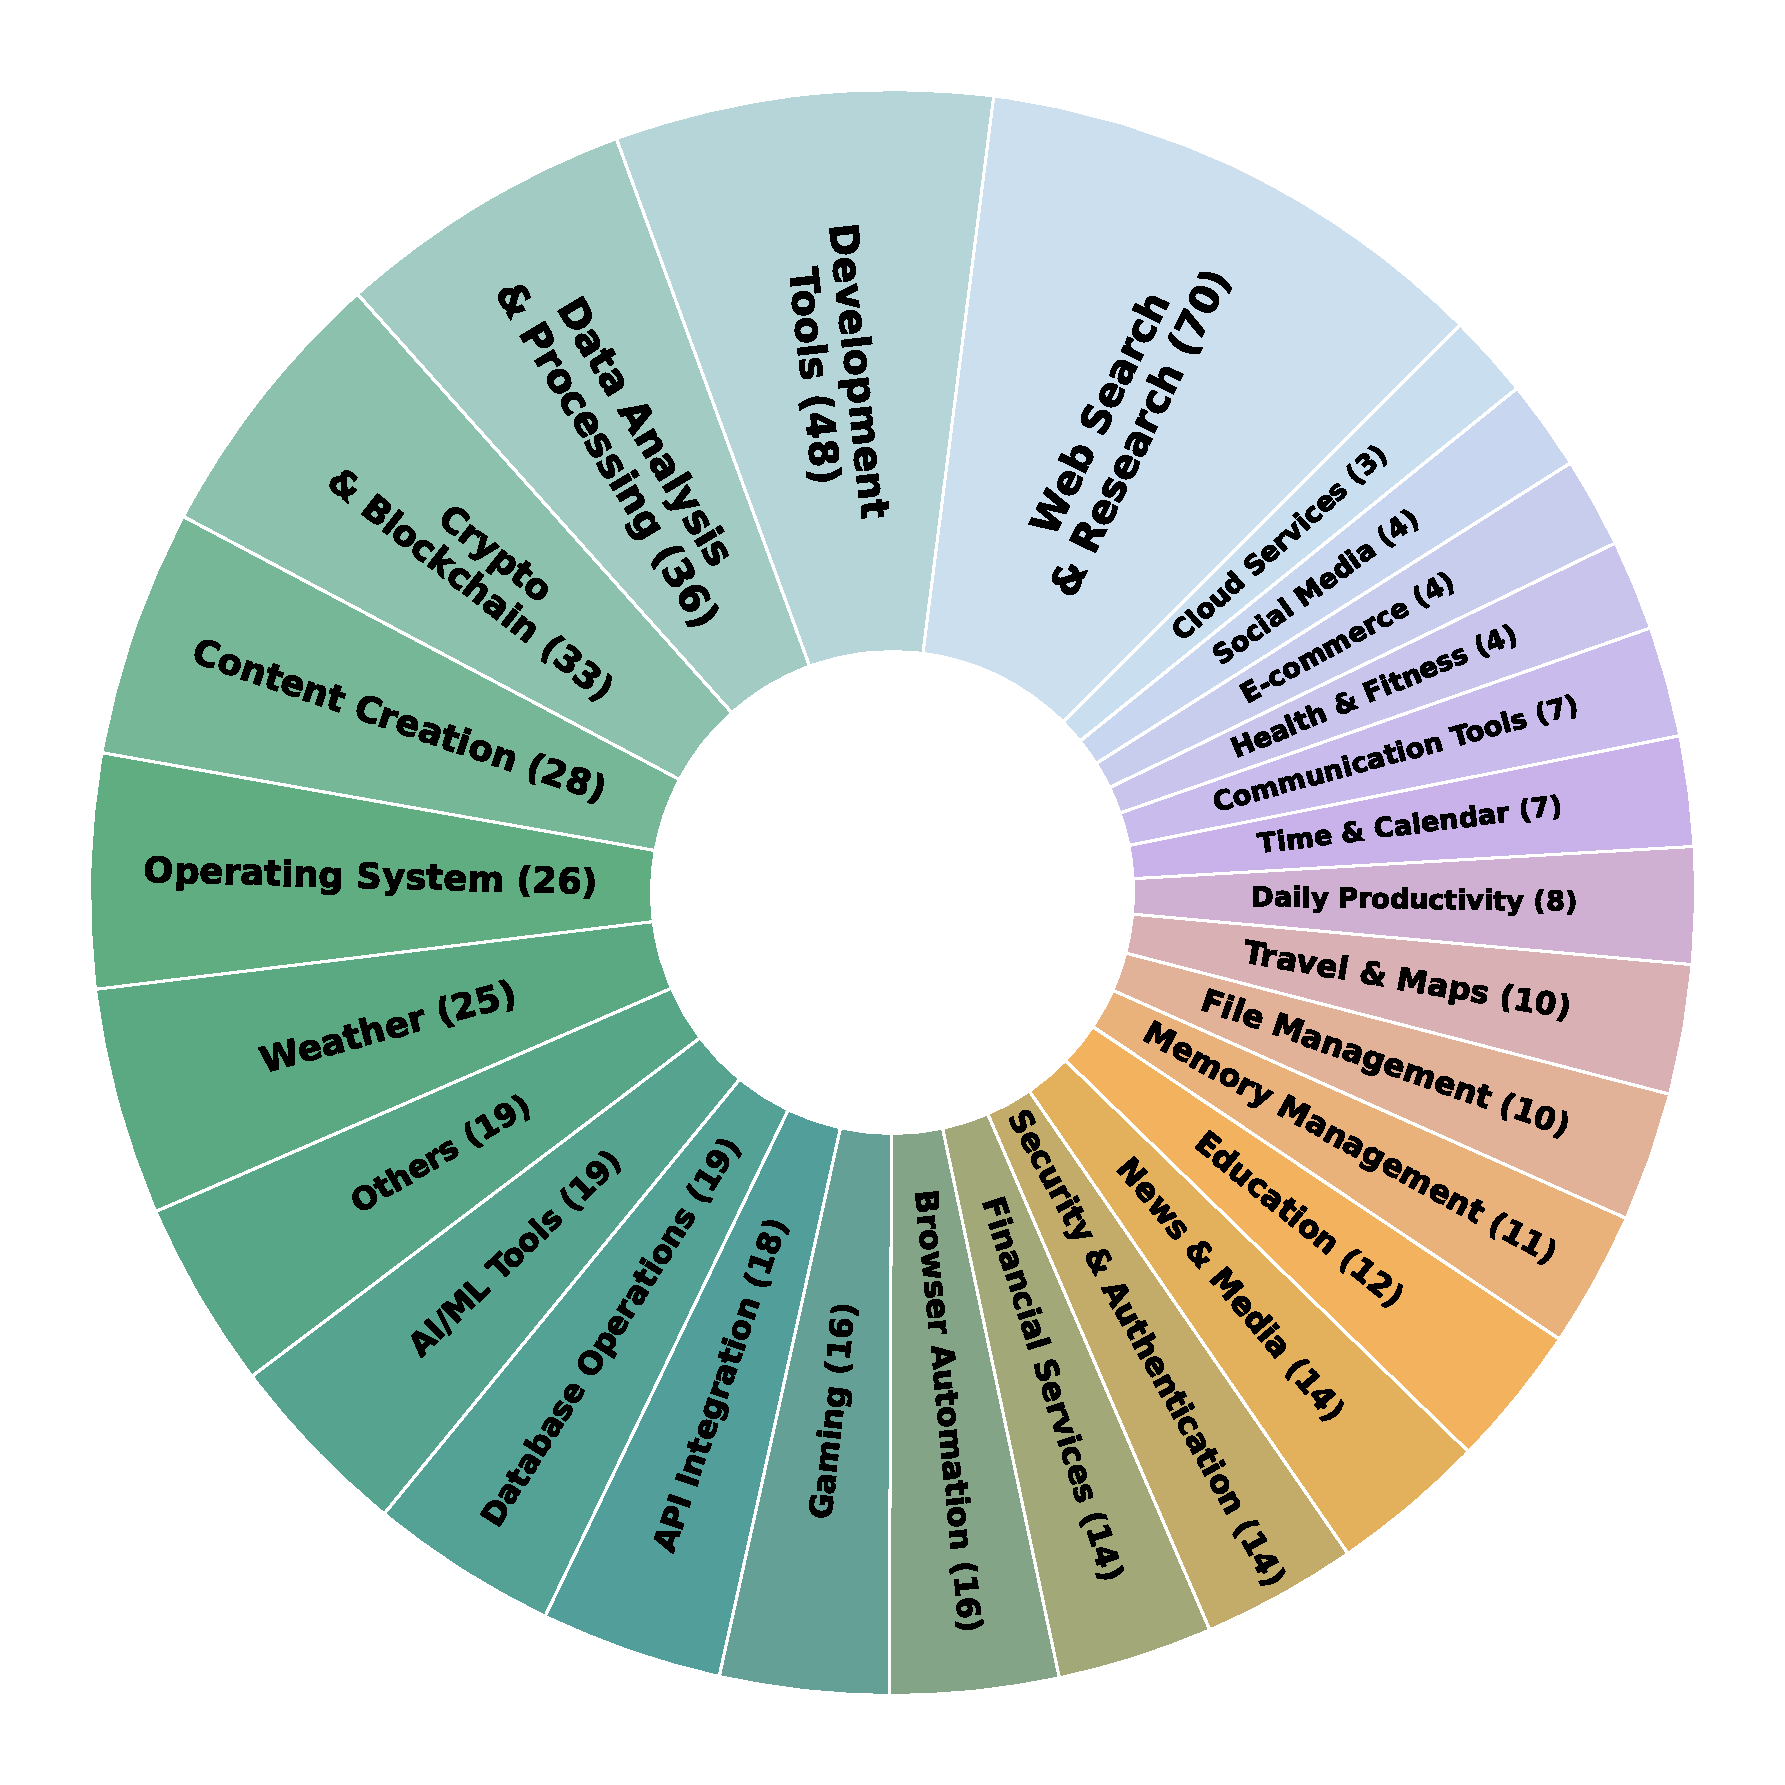
\includegraphics[width=1\linewidth]{images/mcp_primary_labels_ring_internal.pdf}
  \vspace{-0.5em}
  \caption{MCP servers distribution by domain, covering a wide range of categories. Values in parentheses indicate the number of servers belonging to each category.}
  \label{fig:mcp-servers-category}
  \vspace{-2em}
\end{wrapfigure}

% Tool target selection strategies
% Other strategies: persona
% Teacher models

%  \begin{itemize}
%     \item Single server:  single tool, multi-tool; balance distribution according to server usage)
%     \item Multi Server (same category, different category, default as multi-tool)
%     \item Featured Server (a list of aprox. 20 high quality and representative servers, send to LLMs and let it choose whatever makes sense， default as multi-tool)
% \end{itemize}

\textbf{\textcolor{orange!90!black}{Stage 2: Task Synthesis.}} The next step involves synthesizing high-quality tasks from MCP servers, where each task comprises a question and the desired tool names from the MCP servers. The key challenge is ensuring that tasks are challenging, realistic, and cover edge cases. Therefore, we design diverse sampling strategies based on MCP server usage number from Smithery and server functionalities. To avoid potential bias from individual models, we utilized five open-source LLMs (\texttt{Mistral-Small}, \texttt{DevStral-Small}, \texttt{GPT-OSS}, \texttt{Kimi-K2}, and \texttt{Qwen3-32B}) as task generators to construct synthetic tasks (see the prompts in Appendix~\ref{app:task-generation-prompt-for-single-server}). We apply the following three strategies to synthesize tasks, where the maximum number of tools is set to $N=3$ in our experiments:

\textbf{Single Server:} For a given MCP server, we synthesize tasks requiring the use of 1 to $N$ tools, ensuring a balanced selection distribution guided by server usage statistics to reflect real-world applicability.

\textbf{Multi-Server:} Leveraging LLM-based domain annotations derived from MCP metadata, we first sample $N$ MCP servers from either the same or different categories. We then prompt LLMs to conduct a server analysis, outlining potential workflows that integrate tools across these servers, targeting two to $N$ specific tools, and subsequently generating tasks that leverage functionalities from multiple servers.

\textbf{Featured Server:} Based on the original MCP file metadata, we manually selected 25 representative MCP servers from various domains, with the complete list available in Appendix~\ref{app:featured-server-list}. In this approach, we provide all MCP server metadata within the context, specify an expected number of tools, and allow the LLM to freely explore combinations, devise realistic scenarios, select the necessary tools, and create comprehensive tasks.

\textbf{\textcolor{orange!90!black}{Stage 3: Task Filtering.}} 
% LLM-based annotation: quality, realisim, stability, uniqueness, difficulty
To ensure the quality of synthesized tasks, this stage involves annotating tasks across six dimensions and filter out suboptimal instances. We employed the \texttt{Kimi-K2} model as the annotator, which was selected for its optimal balance between correlation with human annotations and cost efficiency. The correlation statistics are detailed in Appendix~\ref{app:llm-annotation}, and the prompt template is provided in Appendix~\ref{app:task-annotation-prompt-for-single-server}. Each dimension is rated on a 1-5 Likert scale. The detailed evaluation metrics are as follows:

\begin{itemize}[itemsep=0pt, parsep=0pt, topsep=0pt, leftmargin=1em]
\item \textit{Tool Selection Difficulty:} Judges the difficulty of selecting the required tools from provided tools.
\item \textit{Tool Selection Uniqueness:} Assesses the uniqueness of the selected tool combination relative to the available tools, and whether viable alternatives could also solve the task.
\item \textit{Question Quality:} The task's overall quality, reflected by its clarity, specificity, and effectiveness.
\item \textit{Scenario Realism:} Evaluates the authenticity and realism of the task scenario.
\item \textit{Verifiable:} Evaluates how easily the final model answer can be verified given the question.
\item \textit{Stability:} Evaluates whether tool outputs remain consistent over time, across geolocation, and under stochastic variation.
\end{itemize}

\textbf{\textcolor{orange!90!black}{Stage 4: Trajectory Generation.}}
This step involves collecting trajectories including tool calls, tool responses, and reasoning steps in agentic environments given tasks synthesized and filtered from the previous steps. To ensure diversity, we employed three LLMs from different families (\texttt{GPT-OSS-120B}, \texttt{Kimi-K2}, and \texttt{Qwen3-32B}) in combination with two agent frameworks (\texttt{Qwen-agent} and \texttt{OpenAI-agent}) to produce high-quality agentic trajectories. The models are deployed remotely and accessed by the agent frameworks via streamable HTTP.

\textbf{\textcolor{orange!90!black}{Stage 5: Rule\&LLM-Based Post-Filtering.}}
The trajectory filtering process combines rule-based verifiers with LLM-driven annotations to ensure high quality. Rule-based heuristics exclude trajectories that fail to start the agent or connect successfully with remote MCP servers, do not contain tool calls, exhibit failures in tool responses, or contain local file system paths. We also validate whether the trajectory uses the required tools specified by the task in the correct sequence, and report both the \textit{desired tool use percentage} (coverage of required tools) and \textit{order correctness} (adherence to expected sequence) metrics. We then employ \texttt{GPT-OSS-120B} as a judge to annotate each trajectory in terms of completeness and conciseness. The annotation prompt is provided in Appendix~\ref{app:trajectory-annotation-prompt-for-single-server}, with metric definitions as follows:
\begin{itemize}[itemsep=0pt, parsep=0pt, topsep=0pt, leftmargin=1em]
\item \textit{Completeness:} Judges whether the assistant fulfills the user's request end-to-end.
\item \textit{Conciseness:} Judges whether the task is solved with the minimum necessary steps and verbosity.
\end{itemize}
This dual-stage filtering approach ensures that only high-quality, concise, and executable trajectories are retained in the final dataset.

\subsection{\dataname Extensions}\label{sec:toucan-extensions}

While the core pipeline generates high-quality trajectories, these are single-turn interactions between user and agent without follow-ups, which limits their practical applicability to real-world scenarios. In addition, since all available tools are contextually relevant, tool selection becomes trivial for LLMs, resulting in relatively low difficulty. To address these limitations and enhance the dataset's versatility, we apply three distinct procedures post-core pipeline (Steps 1 to 5) to generate new instances targeting specific objectives.

\textbf{\textcolor{blue!60!black}{Ext.1: Irrelevance.}} To reduce hallucination, it is critical to train models to reject unanswerable queries or seek alternative solutions when desired tools are unavailable. To achieve this, we systematically generate queries unsolvable with the current toolset (Ext1 in Figure~\ref{fig:toucan-mcp-pipeline}) by shuffling MCP server metadata across instances and repeating the task generation step.

\textbf{\textcolor{blue!60!black}{Ext.2: Persona-based Diversification.}} We implement persona-based diversification (Ext2 in Figure~\ref{fig:toucan-mcp-pipeline}) to create varied task versions. This involves two strategies: one enhances diversity by introducing new contexts and personas, while the other increases task complexity through additional constraints, all while utilizing the same target tools. This diversification process produces tasks similar yet distinct from those in the core pipeline. The prompts are detailed in Appendix~\ref{app:task-diversification-prompts}.

\textbf{\textcolor{blue!60!black}{Ext.3: Multi-Turn.}} Recognizing that real-world user-agent-tool interactions seldom conform to single-turn conversations \cite{yao2024taubenchbenchmarktoolagentuserinteraction}, we introduce a self-simulation pipeline to generate multi-turn dialogues using the trajectory generation model. This is achieved through two methods: (1) splitting complex tasks requiring multi-tool coordination into sequential sub-questions, and (2) extending existing conversations by providing LLMs with context to formulate follow-up queries.

Finally, we repeat the core pipeline from steps~2 to 5 to build full trajectories with the new tasks. In the case of irrelevant tasks (Ext.1), we tighten trajectory filters to retain only instances with zero tool calls. Together, these data extensions yield a more realistic and robust \dataname dataset that covers all relevant tool-use scenarios and user question styles.

\begin{figure}[t!]
% \vspace{-2em}
    \centering
    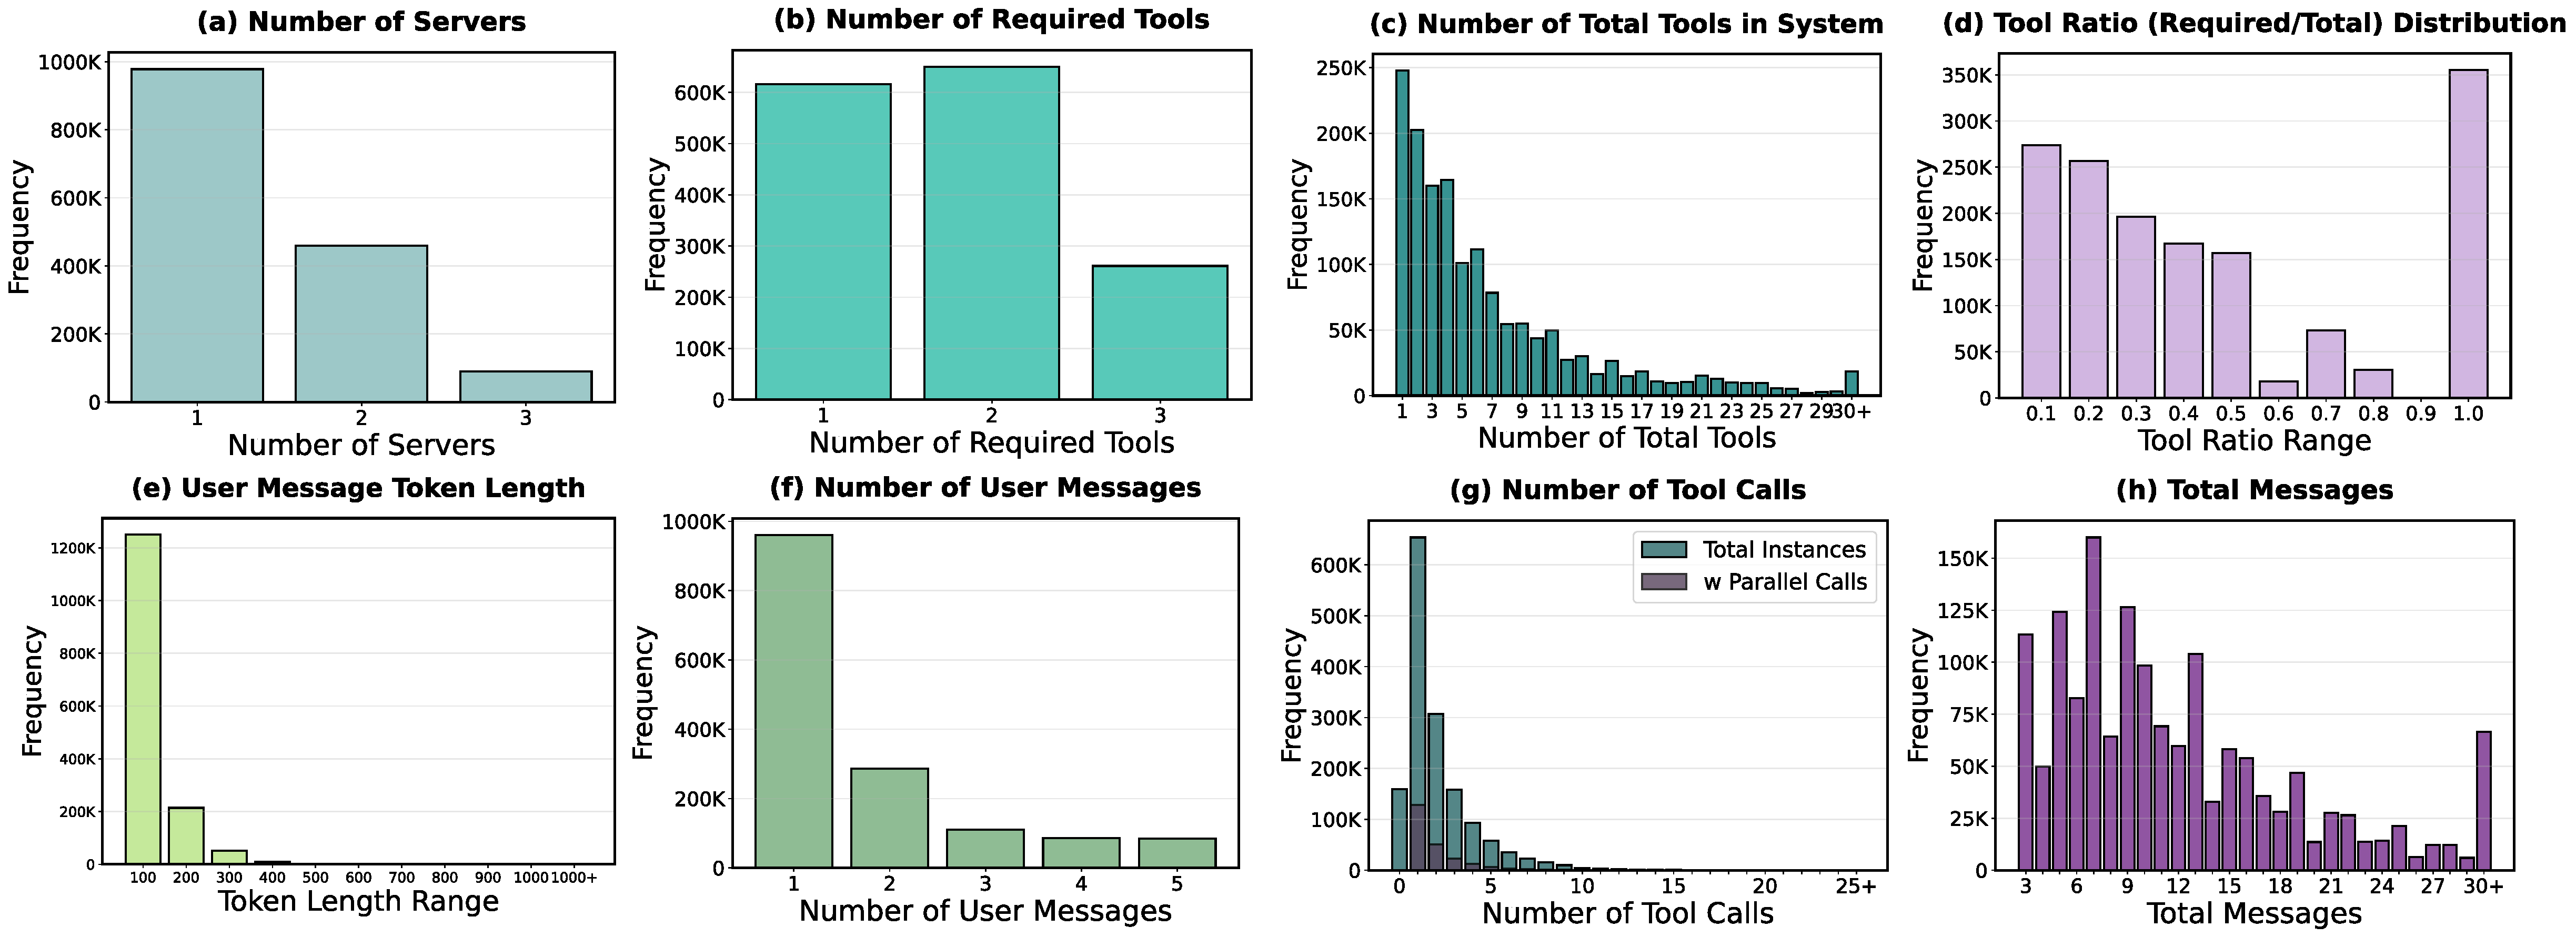
\includegraphics[width=1.0\linewidth]{images/toucan_histo.pdf}
    \caption{The figures above illustrate the \dataname dataset analysis. Subfigure (a) and (b) provide statistics on the number of servers and required tools per instance, highlighting \dataname's comprehensive coverage of multi-server and multi-tool tasks. Subfigures (c) and (d) reveal that most tasks include more tools in the context than the targeted tools, underscoring the non-trivial tool selection challenges. Subfigure (e) displays the length of user messages in tokens. Subfigures (f) and (h) demonstrate the multi-turn nature of the tasks, characterized by extended and diverse interactions among users, agents, and tools. Subfigure (g) demonstrates that \dataname encompasses both single and parallel tool calls, which enhance the dataset's versatility in capturing diverse agent-tool interaction patterns.}
    \label{fig:toucan-dataset-analysis}
    \vspace{-1em}
\end{figure}

\begin{figure}[h]
    \centering
    \begin{minipage}[t]{0.41\textwidth}
        \centering
        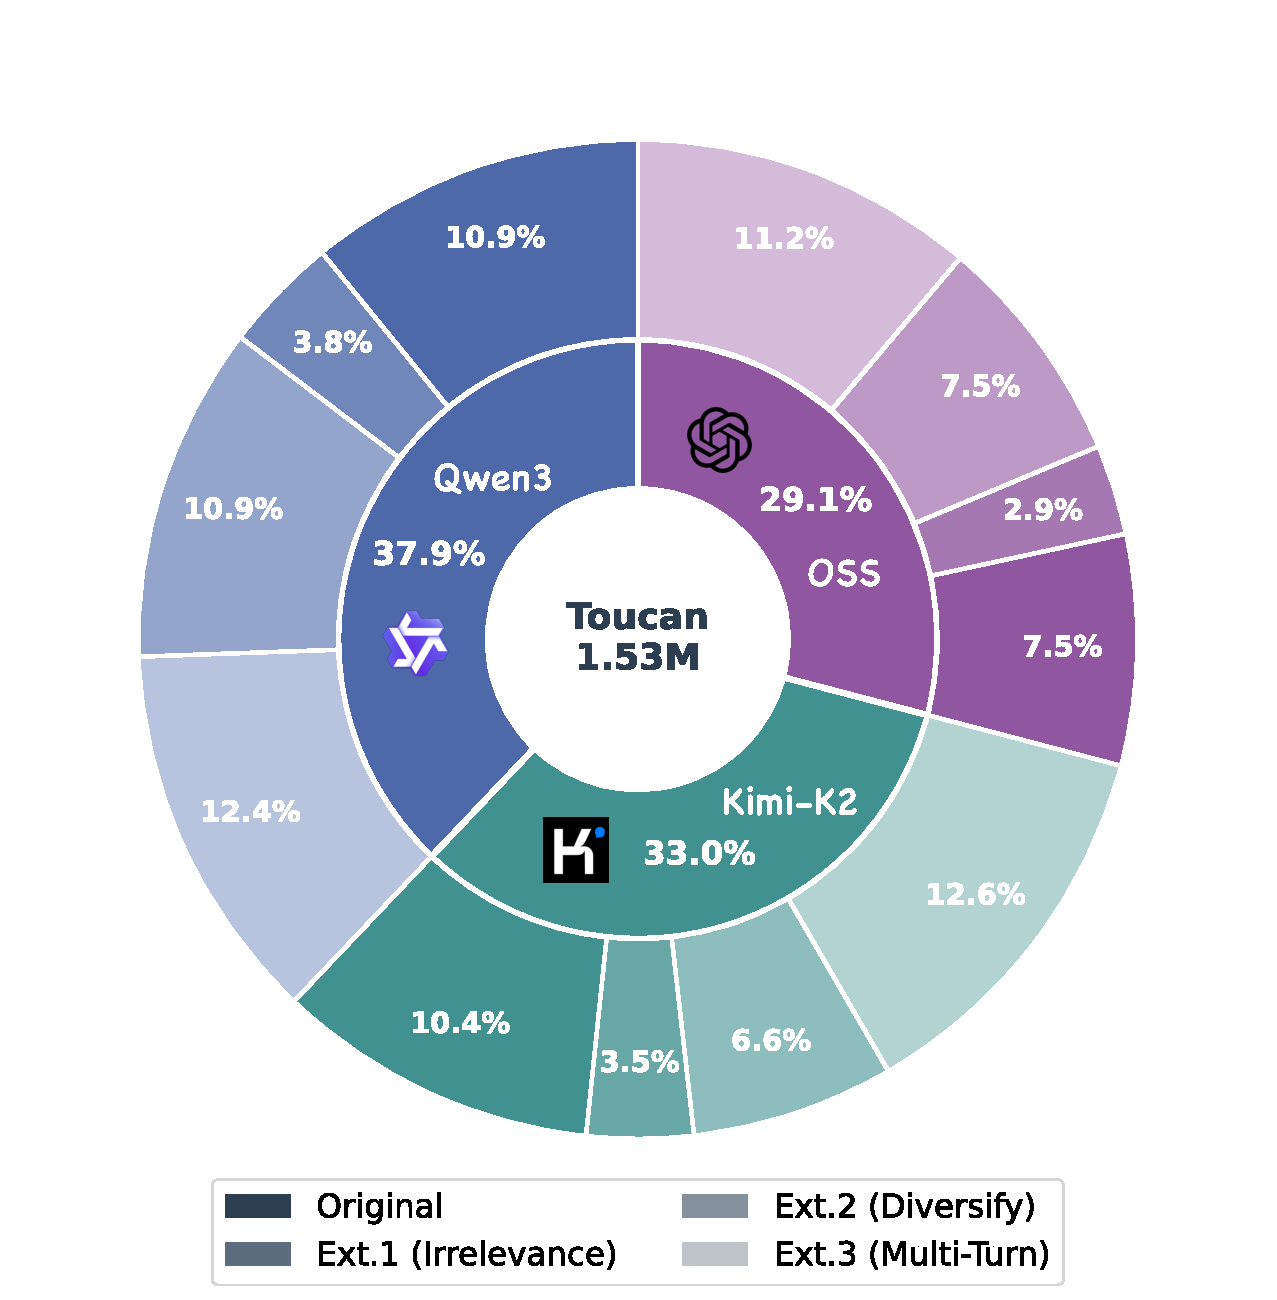
\includegraphics[width=\linewidth]{images/toucan_subset_stats.pdf}
        \caption{\dataname Subset Statistics}
        \label{fig:toucan-subset-stats}
    \end{minipage}
    \hfill
    \begin{minipage}[t]{0.58\textwidth}
        \centering
        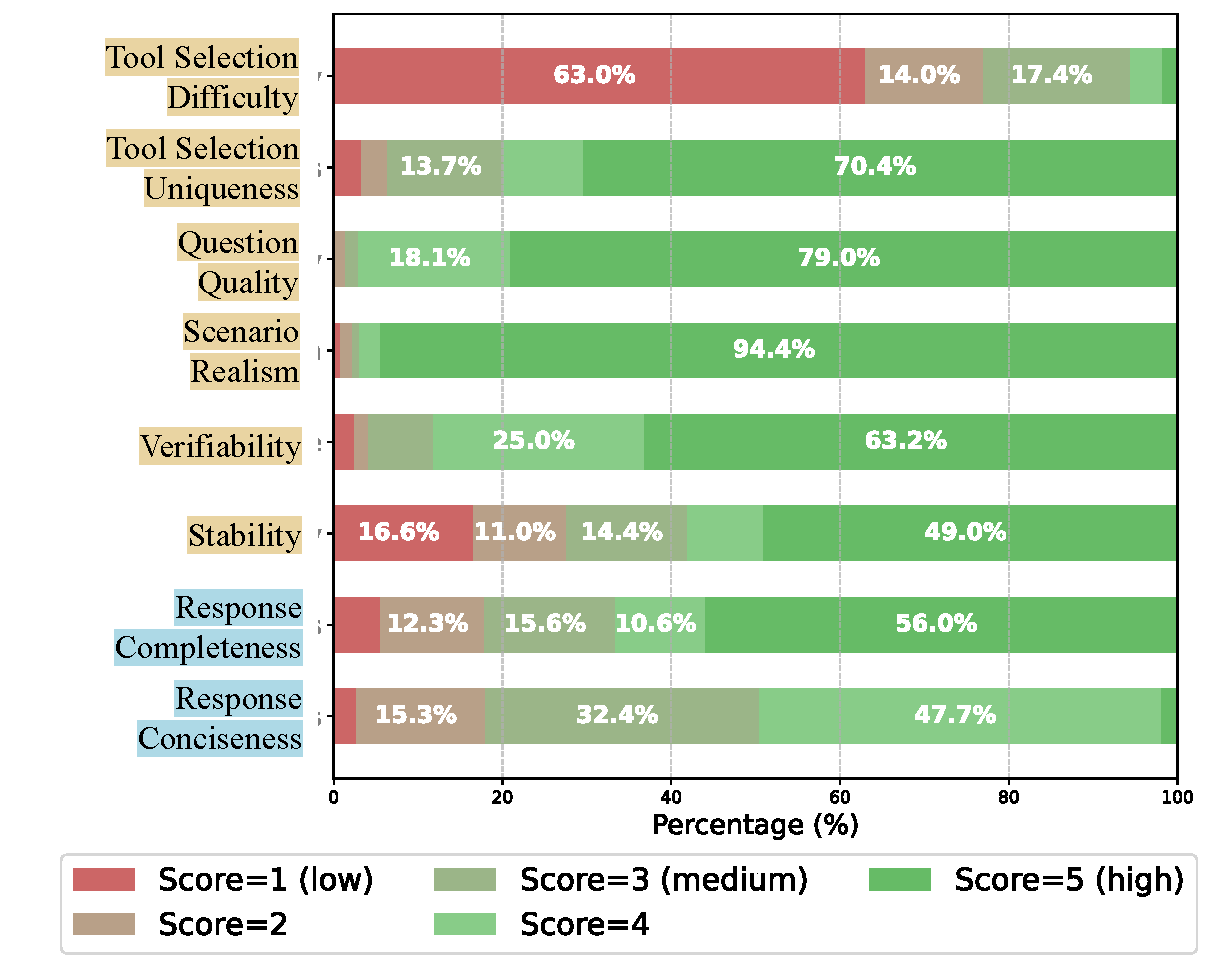
\includegraphics[width=\linewidth]{images/quality_assessment_distribution.pdf}
        \caption{\dataname Quality Statistics}
        \label{fig:toucan-quality-analysis}
    \end{minipage}
    \vspace{-0.5em}
\end{figure}

\subsection{Data Analysis}

This section analyzes the generated \dataname dataset from statistical analysis and LLM-based quality assessment.

\textbf{Statistical Analysis of \dataname.} We conduct comprehensive statistical analysis of MCP servers and data instances. The top MCP servers used in \dataname and tool statistics within each MCP servers are presented in Appendix~\ref{app:top-mcps}. Figure~\ref{fig:toucan-dataset-analysis} provides a comprehensive analysis of the \dataname dataset. We observe that \dataname provides comprehensive coverage of multi-server and multi-tool tasks, and includes multi-turn conversations among users, agents, and tools. Additionally, most tasks contain more tools in the context than the required target tools, indicating non-trivial tool selection requirements. 
Figure~\ref{fig:toucan-subset-stats} presents the subset statistics of \dataname across different trajectory generator LLMs and data partitions.
We also provide embedding visualization of \dataname using UMAP projection in Appendix~\ref{app:embedding-visualization}, demonstrating the wide domain coverage of \datanamen.

\textbf{Quality Assessment of \datanamen.} Figure \ref{fig:toucan-quality-analysis} presents a statistical analysis conducted by an LLM-as-a-judge on \datanamen. From the task perspective (labels in \raisebox{3pt}{\colorbox{taskannocolor}{}}), we observe that the majority of tasks exhibit exceptionally high question quality and scenario realism, indicating robust task design and alignment with real-world applications. Additionally, the dataset features a mixed difficulty range, encompassing both simple and challenging tasks. From the response perspective (label in \raisebox{3pt}{\colorbox{trajannocolor}{}}), we find that trajectory quality is satisfactory, with most scores at or above 3 (medium) across both completeness and conciseness metrics.


